\documentclass[a4paper,12pt]{article} % Prepara un documento per carta A4, con un bel font grande

% impostazioni generali del documento, valide per tutti gli scritti.

\usepackage{graphicx} % per l'inserimento di immagini.

\usepackage[italian]{babel} % Adatta LaTeX alle convenzioni tipografiche italiane,
% e ridefinisce alcuni titoli in italiano, come "Capitolo" al posto di "Chapter", se il vostro documento in italiano
\usepackage[utf8]{inputenc} % Consente l'uso caratteri accentati italiani


\usepackage{fancyhdr} % per il controllo delle intestazioni.
\usepackage{totpages} % macro per conoscere il tatale delle pagine
\usepackage{longtable} % tabelle che vanno su pi� pagine
\frenchspacing % forza LaTeX ad una spaziatura fra parole non inglesi

\pagestyle{fancy}

\newcommand{\linkref}[1]{{\footnotesize \textsl{#1}}}


% fine delle impostazioni generali

\newtoks\titolo % definisco un nuovo comando \titolo che restituisce il titolo.
\newtoks\versione % definisco un nuovo comando \versione che restituisce il versione.
\newtoks\data   % definisco un nuovo comando \data che restituisce la data.

\titolo={Port scans detector with prolog} % inserire qui il titolo

\data={\today}       % today restituisce il valore del giorno in cui si genera il pdf.

\title{\bf \the\titolo}
\author{}
\date{\the\data}


\chead{}

%\lhead{\includegraphics[height=1cm]{logo.png}}
\chead{}
%\lhead{\includegraphics[height=1cm]{../common/logo2.png}}
\rhead{\the\titolo}
\lfoot{Andrea Imparato\\}
\cfoot{\thepage/\pageref{TotPages}}
\rfoot{imparato.andrea@gmail.com}
%\renewcommand{\headrulewidth}{0.4pt} 
%\renewcommand{\footrulewidth}{0.4pt} 
\catcode`\�=\active \def �{\`{\i}}
\catcode`\�=\active \def �{\'{\i}}
\catcode`\�=\active \def �{\`e}
\catcode`\�=\active \def �{\'e}
\catcode`\�=\active \def �{\`E}
\catcode`\�=\active \def �{\'E}
\catcode`\�=\active \def �{\`a}
\catcode`\�=\active \def �{\'a}
\catcode`\�=\active \def �{\`A}
\catcode`\�=\active \def �{\'A}
\catcode`\�=\active \def �{\`u}
\catcode`\�=\active \def �{\'u}
\catcode`\�=\active \def �{\`o}
\catcode`\�=\active \def �{\'o}
\usepackage{xcolor}
\usepackage{multirow}
\definecolor{altncolor}{rgb}{1,1,1}
\usepackage[linkbordercolor=altncolor]{hyperref}
%definizioni per gli url
\usepackage{hyperref} 
\makeatletter
\def\url@leostyle{%
  \@ifundefined{selectfont}{\def\UrlFont{\sf}}{\def\UrlFont{\small\ttfamily}}}
\makeatother
\urlstyle{leo}
%fullscreen
%\hypersetup{backref, pdfpagemode=FullScreen, colorlinks=false, urlbordercolor= altncolor} 
\hypersetup{backref, colorlinks=false, urlbordercolor= altncolor} 

 % inserisco le intestazioni del doc: logo, nome etc..

\begin{document}


\begin{titlepage} % inizio la pagina che contiene il titolo.

\begin{center}


	 
\includegraphics[height=5cm]{logo_unipd.png}\\[1cm]
	   %\includegraphics{logo_uni.png}\\[2cm]
	    \huge \textbf{\the\titolo}\\[7cm]


	\large \emph{Progetto per il corso di intelligenza artificiale anno 2010/2011}\\[1cm]
	\normalsize \textbf{Andrea Imparato} % Redattori o Redattore
	\normalsize \textbf{Matricola 623480}


\end{center}
\end{titlepage}



\newpage

\tableofcontents

\newpage

\section{Introduzione}

In questo progetto è stato realizzato un \emph{port scanners detector} che utilizza \textbf{Prolog} per il riconoscimento
di un port scanning.\\

Il port scanning è una tecnica che viene utilizzata per l'identificazione delle porte "aperte" in un host remoto.
Come si sa, infatti, quando si apre un servizio questo si mette in ascolto su una determinata porta, assegnata dal sistema 
operativo, delle connessioni in entrata.

Alcuni di questi servizi molto spesso possono essere vulnerabili e quindi sfruttabili dall'esterno per ottenere accesso
non autorizzato. Il \emph{port scanning} viene utilizzato dunque per il riconoscimento di quali servizi sono attivi ed
è il primo passo infatti prima di un eventuale attacco.\\


Esistono vari software sul mercato che eseguono l'analisi degli host di una rete per il riconoscimento di intrusioni 
non autorizzate e vengono chiamati \emph{Intrusion detection systems}. Questi software possono essere molto evoluti 
e sfruttare tecniche di \emph{intelligenza artificiale} o \emph{apprendimento automatico} per le loro attività che possono essere analisi del traffico di rete, dei log oppure del carico cpu o I/O del sistema. All'interno di questi software è 
presente un modulo per il riconoscimento di scansioni di porte. \\

In questo progetto si è voluto realizzare uno di questi possibili moduli utilizzando una base di conoscenza
realizzata in \emph{Prolog}.  



\section{Consuntivo}

Per la realizzazione del progetto sono state impiegate all'incirca 100 ore complessive distribuite in questo modo:

\begin{itemize}

\item 50 ore per lo studio della progettazione e lo studio delle tecnologie da utilizzare nel progetto
\item 40 ore per lo sviluppo 
\item 10 ore per la stesura di questa relazione


\end{itemize}


\newpage

\section{Use case}

Sono stati progettati 2 casi d'uso principali:
\begin{figure}[htbp]
 \begin{center}
  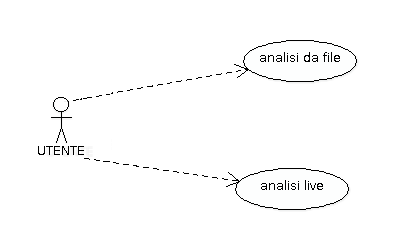
\includegraphics[width=15cm]{usecase1.png}
  \end{center}
  \caption{\label{fig_caso_generale} Casi d'uso}
 \end{figure}\\


\begin{itemize}


\item analisi \textbf{offline} da file: l'utente puo' far analizzare un file di traffico precedentemente catturato. In gergo
il traffico viene "sniffato", vengono catturati i pacchetti e salvati su file. I programmi maggiormente utilizzati per la cattura sono \textbf{tcpdump} e \textbf{Wireshark}. Il primo esegue da riga di comando e il secondo è una sua interfaccia grafica. Dopo aver catturato il traffico, l'utente esegue l'analisi del file e il sistema riporta 
la presenza o meno di un port scanning da parte di un host remoto e il suo indirizzi ip.

\item analisi \textbf{online} del traffico di rete: l'utente esegue il software che effettua lo "sniffing" live 
del traffico e in modo continuativo la sua analisi. Se viene rilevato uno scanning il sistema esce e riporta la presenza dello scannning e dell'host remoto che l'ha eseguito e il suo indirizzo ip. 

\end{itemize}









\section{Scenari}






\section{Progettazione}


\section{Tecnologie}


\section{Inferenza}


\section{Risultati}



\section{Sviluppi futuri}
\end{document}
